% Chapter Template

\chapter{Definición del problema}

\label{Chapter5} % Change X to a consecutive number; for referencing this chapter elsewhere, use \ref{ChapterX}

\section{Kaggle}

En el año 2007, \textit{Netflix} creó una competición para mejorar su motor de
recomendación de películas. Publicó un conjunto de datos las películas elegidas
por los diferentes usuarios y pidió a los participantes realizar un modelo
predictivo usando este conjunto de datos. Evaluaron los modelos predictivos
presentados usando un conjunto de datos diferente y otorgaron el premio al que
menos error presentaba. El premio para el mejor modelo predictivo era de un
millón de dólares.

En 2010 el economista australiano Anthony Goldbloom, inspirándose en la idea de
la competición de Netflix, creó \textit{Kaggle}. \textit{Kaggle} es una
plataforma de competiciones de análisis y modelización predictiva de datos.

El funcionamiento de la plataforma consiste en lo siguiente: un equipo promotor
contacta con \textit{Kaggle} y prepara un conjunto de datos para la competición.
Un subconjunto de esos datos son publicados en la web para el uso de los
participantes. El otro subconjunto, oculto, se usa para determinar el mejor
modelo presentado y declarar un ganador.

El conjunto de datos presentado contiene las respuestas de cada elemento
(permitiendo así que los modelos usen aprendizaje supervisado). Junto a los
datos se especifica una métrica que servirá para medir la bondad del modelo.

Para presentar el modelo el participante debe presentar las predicciones del
conjunto de test en la web de \textit{Kaggle}. La puntuación obtenida según la
métrica sobre una parte del conjunto de test se hará pública en la tabla de
posiciones pública. Cuando la competición termina se genera una tabla de
posiciones privada, donde se publica a la puntuación del modelo usando el
conjunto de test completo, y es con esta puntuación con la que se determina el
ganador. Se hace de esta manera para evitar que los participantes sobreajusten
el modelo al conjunto de test.

Existen varios tipos de competiciones a las que los usuarios se pueden
presentar:

\begin{itemize}
  \item \textit{\textbf{Getting started}}: Competiciones sencillas organizadas por la
      misma plataforma con la finalidad de que los usuarios se familiaricen con
      los modelos predictivos y la estructura de las competiciones. Suelen tener
      un conjunto de datos ordenado y sencillo, y existe mucha documentación y
      ayuda en los foros.
  \item \textit{\textbf{Playground}}: Competiciones que no resuelven problemas
      reales, diseñadas para que los usuarios experimenten y prueben diferentes
      ideas. No tienen ningún premio.
  \item \textit{\textbf{Research}}: El objetivo de estas competiciones es la
      investigación sobre diferentes técnicas o de problemas de bien común.
      Muchas de estas competiciones tienen como premio la invitación a
      conferencias o a publicar los resultados en algún medio. Suelen requerir
      que las soluciones sean publicadas como código abierto.
  \item \textit{\textbf{Recruiting}}: Los organizadores de estas competiciones
      buscan contratar a los mejores participantes.
  \item \textit{\textbf{Featured}}: Las competiciones con más dificultad y
      mejores premios. Buscan resolver un problema real y posiblemente
      comercial. Aquí entraría la competición de Netflix.
\end{itemize}

A principios de 2017 \textit{Kaggle} fué comprado por \textit{Google}, aunque por ahora sigue siendo una
plataforma independiente funcionando bajo su propio nombre.

\section{\textit{ The Nature Conservancy Fisheries Monitoring }}

En el océano pacífico, donde se captura más del 60\% del atún del mundo, tienen lugar prácticas de pesca irregular que amenazan a los ecosistemas marinos y a la estabilidad de la pesca mundial. \textit{The Nature Conservancy} es una asociación que trabaja con organizaciones locales y globales para preservar las especies marinas de cara al futuro.

La principal idea para controlar la pesca y explotación de recursos marinos es el uso de cámaras en barcos, que ayudan a monitorizar las actividades pesqueras de estos. Aunque funciona muy bien como sistema de control, la cantidad de datos e imágenes generadas hace que sea muy costoso de procesar manualmente.

\begin{figure}
  \centering
  \caption{\textit{Ejemplo de imágenes tomadas en barcos pesqueros para su posterior identificación}}
\label{kaggle-banner}
  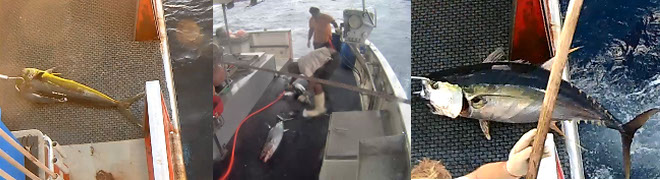
\includegraphics[width=\textwidth]{kaggle-competition-banner}
\end{figure}

La idea de este reto es desarrollar algoritmos que detecten y clasifiquen automáticamente especies de atunes, tiburones y otras especies que estos barcos pesqueros cazan. El que se pueda analizar imágenes como las de la figura \ref{kaggle-banner} de una manera rápida y automática permitirá asignar recursos de una manera mucho más efectiva para el control de este tipo de actividades \parencite{kaggle-page}.

\section{Definición del problema}

El problema consiste en clasificar cada una de las imágenes de un conjunto de imágenes de barcos en una de las ocho categorías disponibles. Las imágenes suelen mostrar la cubierta de un barco donde puede aparecer un pez. En base al pez que aparezca hay que clasificarlo en una de las seis categorías mostradas en la figura:

\begin{figure}
  \centering
  \caption{Especies de peces a clasificar en el reto}
\label{kaggle-fishes}
  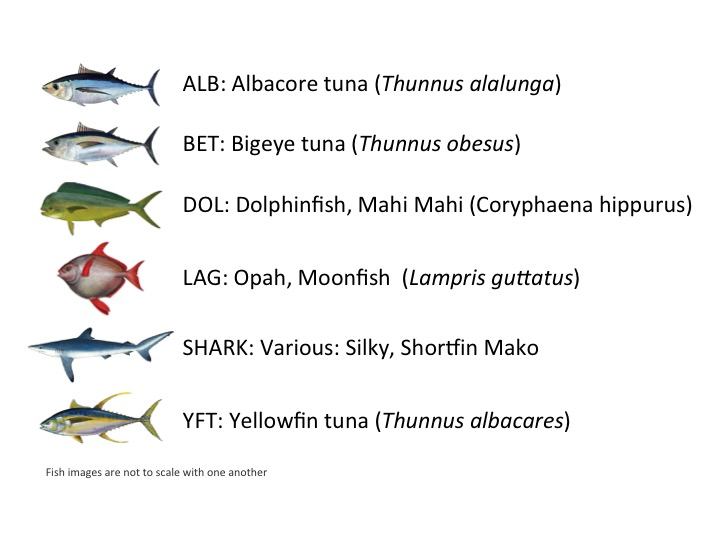
\includegraphics[width=\textwidth]{species-ref-key}
\end{figure}

En caso de que no aparezca ningún pez en la imagen, esta tendrá la categoría NOF (\textit{No Fish}). Y si aparece un pez en la imagen pero no perteneciente a ninguna de las categorías mencionadas, la categoría será OTHER.

En resumen, el conjunto de posibles categorías es:
\[
  categories =
  \left[ALB, BET, DOL, LAG, SHARK, YFT, OTHER, NOF]
\]

\subsection{Datos}

La competición proporciona tres ficheros con los que trabajar:

\begin{enumerate}
  \item{Conjunto de datos de entrenamiento: 3777 imágenes etiquetadas con una de las ocho categorías existentes.}
  \item{Conjunto de test y evaluación: 1000 imágenes sin etiquetar.}
  \item{Archivo de envío de prueba: Archivo CSV que muestra la estructura que debe tener el archivo con las soluciones}
\end{enumerate}

\subsection{Envío de la solución y evaluación}
\label{sec:envio-y-eval}

Para el envío de la solución hace falta clasificar las 1000 imágenes del conjunto de evaluación, indicando la probabilidad de que caiga en cada una de las ocho categorías diferentes. En la tabla \ref{submission-sample} se muestra un ejemplo de las primeras filas del archivo CSV a enviar.

\begin{table}[]
\centering
\caption{Ejemplo del archivo de envío}
\label{submission-sample}
\begin{tabular}{lllllllll}
image          & ALB   & BET   & DOL   & LAG    & NoF   & OTHER & SHARK  & YFT  \\
img\_00005.jpg & 0.455 & 0.052 & 0.030 & 0.0173 & 0.123 & 0.079 & 0.046 & 0.194\\
img\_00007.jpg & 0.455 & 0.052 & 0.030 & 0.0173 & 0.123 & 0.079 & 0.046 & 0.194\\
img\_00009.jpg & 0.455 & 0.052 & 0.030 & 0.0173 & 0.123 & 0.079 & 0.046 & 0.194
\end{tabular}
\end{table}

Los resultados enviados se evalúan mediante una función de pérdida logarítmica multiclase. Concretamente se usa la fórmula:
\[
  logloss =
  - \frac{1}{N} \sum_{i=1}^N \sum_{j=1}^M y_{ij} \log \, p_{ij}
\]
 siendo N el número de imágenes en el conjunto de test, M el número de categorías, $y_{ij}$ 1 si la observación $i$ pertenece a la clase $j$ y 0 si no pertenece y $p_{ij}$ la probabilidad predicha de que el elemento $i$ pertenezca a la clase $j$.

 \subsection{Leaderboard y fases de la competición}

Cuando un participante envía una predicción, \textit{Kaggle }calcula la puntuación de dicho envío sobre un subconjunto del conjunto de test, mostrando la puntuación en una tabla de clasificación pública. Se usa un subconjunto para enviar que los participantes puedan aprovechar un sobreajuste a la hora de entrenar el modelo. Al llegar a la fecha de entrega de las predicciones y modelos se recalculará esta tabla con todo el conjunto de test.

Antes de terminar la primera fase de la competición los participantes deberán subir a \textit{Kaggle} el modelo utilizado y seleccionar las dos predicciones que quieren usar para la puntuación con el conjunto completo. La puntuación de estas predicciones se hará usando todo el conjunto de test y se publicará en una tabla de clasificación privada, solo visible para los participantes. 

Una vez terminada la primera fase, \textit{Kaggle} publicará un nuevo conjunto de test, con el que los participantes deberán clasificar usando el modelo entregado al final de la fase anterior.

En esta segunda fase, que dura solo cinco días, el procedimiento es el mismo. Se publicarán puntuaciones usando un subconjunto del segundo conjunto de test y al terminar se publicará la puntuación usando el conjunto completo. Esta última puntuación será la puntuación final de la competición. Si alguno de los participantes ha hecho un envío en la primera fase pero no ha hecho ninguno en la segunda, quedará eliminado de la competición.

\section{El conjunto de datos}

Aqui hago un pequeño análisis del conjunto de datos, la distribución de imágenes por clases, por estructura (tamaño de imaggen), color, etc

